\documentclass[conference]{IEEEtran}

\usepackage{amsmath}
\usepackage{graphicx}
%\usepackage[backend=bibtex,style=chem-rsc]{biblatex}
\usepackage{lettrine}
\usepackage{cite}
\usepackage{float}
\usepackage{blindtext}
\usepackage{eso-pic}
\usepackage[utf8]{inputenc}
\usepackage[english]{babel}
\usepackage[numbers]{natbib}
\usepackage{hyperref}
\usepackage{booktabs}
\usepackage{filecontents}
\newcommand\tab[1][1cm]{\hspace*{#1}}
\newcommand\AtPageUpperMyright[1]{\AtPageUpperLeft{%
    \put(\LenToUnit{0.5\paperwidth},\LenToUnit{-1cm}){%
     \parbox{0.5\textwidth}{\raggedleft\fontsize{9}{11}\selectfont #1}}%
    }}%
    \newcommand{\conf}[1]{%
    \AddToShipoutPictureBG*{%
    \AtPageUpperMyright{#1}}
}

\title{Sample paper}

\author{
  \IEEEauthorblockN{Armaan Kohli}
  \IEEEauthorblockA{\textit{Department of Electrical Engineering} \\
\textit{The Cooper Union for the Advancement of Science and Art}\\
New York City, United States \\
kohli@cooper.edu\\
\href{github.com/armaank/wi-comms}{https://github.com/armaank/wi-comms}}}

\begin{document}
\title{Rayleigh Flat-Fading Mitigation via Alamouti Codes}

\maketitle
\conf{ECE-408: WIRELESS COMMUNICATIONS, MARCH 2020}

\begin{abstract}
 We simulate a wireless link over a Rayleigh channel, and compare the bit-error-rate (BER) performance of different diversity schemes. Specifically, we compare coherent binary phase shift keying (BPSK) with maximal-ratio-reciever combiner (MRRC) schemes and two-branch transmit diversity schemes via Alamouti codes. In this project, we demonstrate an understanding of how diversity techniques can correct Rayleigh fading channels.
\end{abstract}

\begin{IEEEkeywords}
Rayleigh fading, maximal ratio combining, transmit diversity, wireless link simulations
\end{IEEEkeywords}

\section{Introduction}
\lettrine[findent=2pt]{\textbf{O}}{ }ne of the most important problems in wireless communications regards communication through multi-path fading channels. Rayleigh fading channels are commonly used to model communications between moving mobile devices. Before Siavash Alamouti \cite{alamouti}, methods used to mitigate such degenerate channels included increasing transmit power (or bandwidth), time and frequency diversity. While time and frequency diversity techniques were promising, they were in some cases ineffective, and often required more complex, and thus more expensive receivers. As such, antenna diversity was a promising alternative. One common approach to antenna diversity was maximal-ratio receiver combining (MRRC). This approach, however, required multiple antennas at the receiver. Alamouti, however, proposed a new type of antenna diversity, on the transmitter side that could achieve the same performance as MRRC. We simulate an uncoded binary phase shift keying (BPSK) signal, as well as both MRRC and Alamouti diversity techniques over a Rayleigh flat-fading channel in order to evaluate the performance of the scheme proposed by Alamouti and to learn about multi-path channel models and how to mitigate their effects on signal integrity. 

\section{Rayleigh Channel Model}
We simulate a Rayleigh flat-fading channel. First, we generate white complex Gaussian noise. We then filter the white noise through a filter with a frequency response equal to the square root of the required Doppler Spectra. We can compute the Doppler spectrum using the following formula. The spectra is illustrated in Fig. \ref{fig:dop}
\begin{equation}
S_{E_z} = \frac{1.5}{\pi f_d\sqrt{1-\left(\frac{f}{f_d} \right)^2}}
\end{equation}
\begin{figure}[htbp]
\centerline{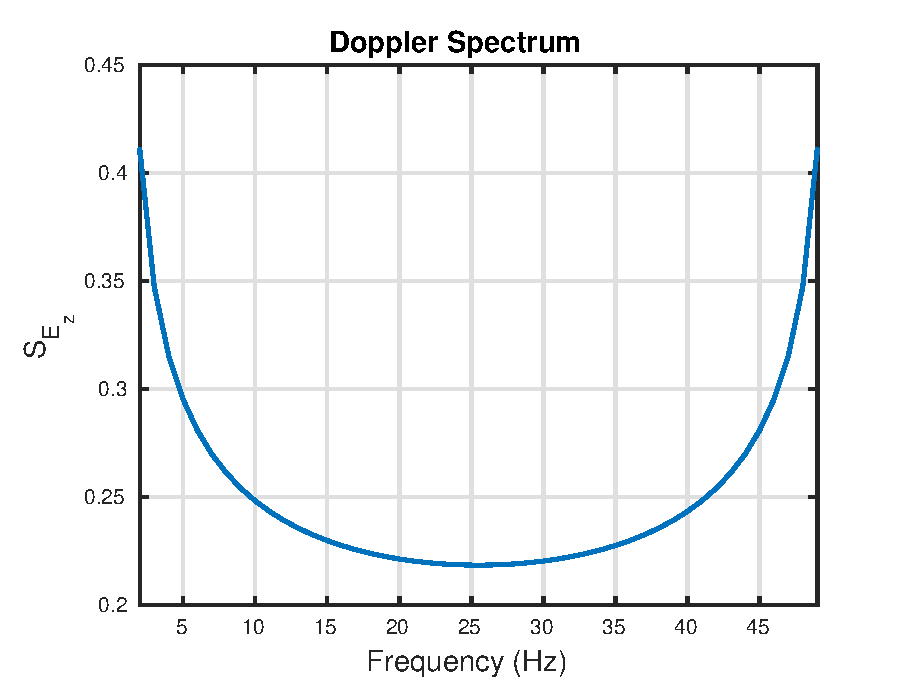
\includegraphics[scale=.5]{./media/doppler.eps}}
\caption{The square-root of the spectra with a Doppler frequency $f_d = 10Hz$. }
\label{fig:dop}
\end{figure}
We filter the white noise samples by multiplying by the required frequency response. We then perform an inverse-fast-Fourier-transform (IFFT) to convert the channel back into the time domain. We then sum the square-roots of our filtered white noise and square the output to generate our channel. A sample Rayleigh flat-fading channel is pictured in Fig \ref{fig:ray}
\begin{figure}[htbp]
\centerline{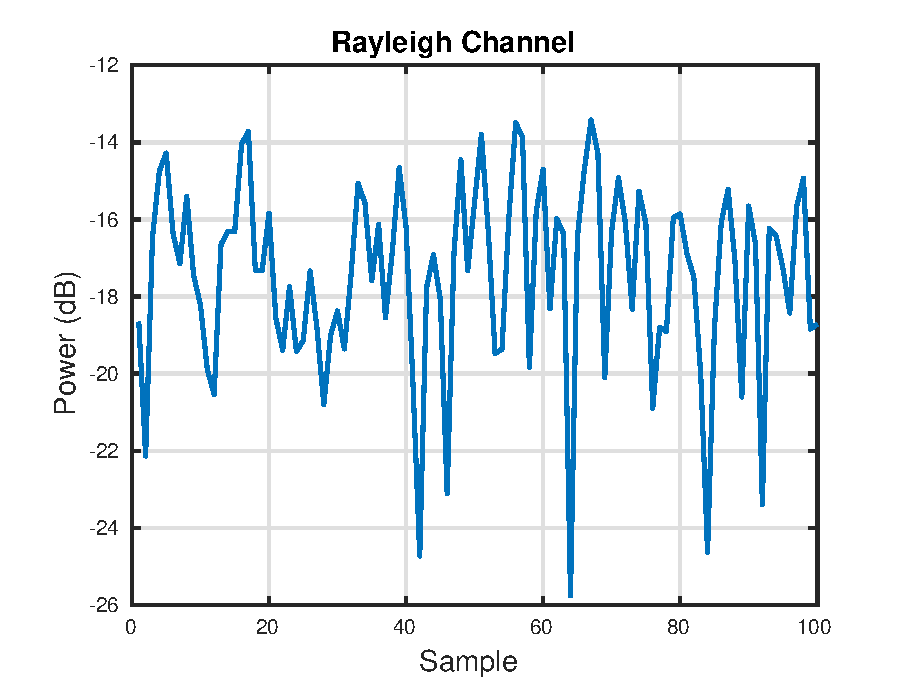
\includegraphics[scale=.5]{./media/raychan.eps}}
\caption{A Rayleigh flat-fading channel with a Doppler frequency $f_d = 10Hz$. }
\label{fig:ray}
\end{figure}

\section{Diversity Techniques}
In order to successfully transmit data through a multi-path channel, we employ two different diversity schemes.
\subsection{MRRC}
MRRC is a receiver-based antenna diversity scheme. The scheme works by combining the received signal from two different antennas and performing maximum likelihood detection. The scheme is illustrated in Fig. \ref{fig:mrrc}, reproduced from \cite{alamouti}. 
\begin{figure}[htbp]
\centerline{\includegraphics[scale=.4]{./media/mrrc.png}}
\caption{Two-branch MRRC}
\label{fig:mrrc}
\end{figure}
\subsection{Alamouti}
The new scheme that Alamouti proposes differs from the conventional MRRC. First, the diversity occurs on the transmit side of the link, making it more efficient to implement practically speaking. At the first time interval, two different symbols are sent on different antennas. The next time interval, the cooresponding symbols are swapped and sent on the opposite antenna. Using an altered combining scheme, the receiver can recover the transmitted symbols with the same maximum likelihood decision role, apart from a noise phase offset, which doesn't impact signal-to-noise ratio (SNR). This technique is illustrated in Fig. \ref{fig:alamouti}, reproduced from \cite{alamouti}.
\begin{figure}[htbp]
\centerline{\includegraphics[scale=.6]{./media/alamouti.png}}
\caption{Transmit diversitiy scheme proposed by Alamouti}
\label{fig:alamouti}
\end{figure}
\section{Simulations and Results} 
We reproduce Fig. 4 from \cite{alamouti} in order to verify the effectiveness of diversity coding as a mitigation technique for multipath channels. First, we simulate uncoded BPSK through the channel. We then implement MRRC with two and four receivers. Finally, we simulate the new scheme proposed by Alamouti with two transmitters and 1 receiver, and two transmitters and two receivers. The simulated BER curves are presented in Fig. \ref{fig:ber}
\begin{figure}[htbp]
\centerline{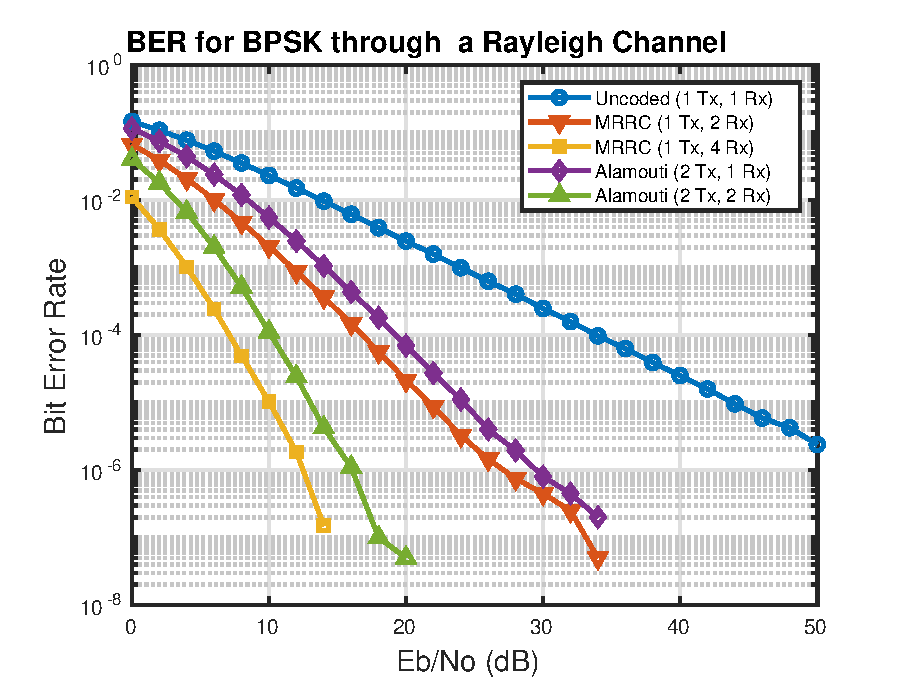
\includegraphics[scale=.6]{./media/ber.eps}}
\caption{Comparing BER of coherent BPSK with MRRC and the new transmit diversity scheme in Rayleigh flat-fading.}
\label{fig:ber}
\end{figure}
As expected performance is worst without any diversity techniques. The MRRC appears to outperform the Alamouti scheme. However, the difference between the two is precisely $3dB$, which comes from the signal power being split in half for each of the two transmit antennas required by the Alamouti technique. Thus, this shows that the new scheme can achieve identical performance to MRRC, without the need to increase the receiver complexity. Furthermore, the $3dB$ difference can be easily solved by the use of two, cheap RF power amplifiers, which combined, would likely cost less than a single, highly-linear RF power amplifier required for MRRC, making the new scheme far more realizable. 

\section{Conclusion} 
We successfully simulated a Rayleigh flat-fading channel and compared various diversity techniques to mitigate the channel. We successfully reproduced Alamouti's results as presented in Fig. 4 from his seminal paper. We learned about channel models and diversity as a way to improve BER performance in wireless settings. 
\bibliographystyle{unsrt}
\bibliography{bibli}
\end{document}